\documentclass{./../Latex/handout}
\begin{document}
\thispagestyle{plain}
\myheader{Comparative Statics}


%%%%%%%%%%%%%%%%%%%%%%%%%%%%%%%%%%%%%% Difference Quotient and the Derivative
\section{Difference Quotient and the Derivative}
We are often interested in how some variable $y$ changes in response to another variable $x$ where:
$$
y=f(x)
$$

To see how $y$ changes with $x$, we can think about how the value of $f(x)$ changes when say $x$ goes from $x_0$ to $x_1$. Denote change in the value of a variable by $\Delta$. Then $\Delta x=x_{1}-x_{0}$. When $x$ changes from an initial value $x_{0}$ to a new value $x_{0}+\Delta x$, the value of the function $y=f(x)$ changes from $f\left(x_{0}\right)$ to $f\left(x_{0}+\Delta x\right)$. The change in $y$ per unit of change in $x$ can be represented by the difference quotient:
$$
\frac{\Delta y}{\Delta x}=\frac{f\left(x_{0}+\Delta x\right)-f\left(x_{0}\right)}{\Delta x} .
$$ \\

\textit{Example.} For the function: $y=f(x)=x^{2}+20$
\begin{align*} \frac{\Delta y}{\Delta x}&=\frac{f\left(x_{0}+\Delta x\right)-f\left(x_{0}\right)}{\Delta x} \\
&= \frac{(x_0+\Delta x)^2+20-(x_0^2+20)}{\Delta x} \\
&= \frac{x_0^2+ (\Delta x)^2+2 x_0 \Delta x-x_0^2}{\Delta x} \\&= 2 x_0 + \Delta x
\end{align*} 

We are usually interested in minuscule changes from $x_0$. The \textit{derivative} of a function is defined as:
$$ \frac{\partial y}{\partial x} = f'(x)= \lim_{\Delta x \rightarrow 0} \frac{\Delta y}{\Delta x} $$
So for the example above:
$$ \frac{d y}{d x} = f'(x_0)= \lim_{\Delta x \rightarrow 0} 2 x_0 + \Delta x = 2 x_0 $$

Note that both the following definitions of the derivative are equivalent:
\begin{align*}
(1). \quad 	\frac{d y}{d x} &= f'(x_0) = \lim_{\Delta x \rightarrow 0} \frac{f\left(x_{0}+\Delta x\right)-f\left(x_{0}\right)}{\Delta x} \\~\\
(2). \quad 	\frac{d y}{d x} &= f'(x_0) = \lim_{ x \rightarrow x_0} \frac{f(x)-f(x_{0})}{x-x_0}  
\end{align*} \\

\textit{Example.} Let's find the derivative of $y=f(x)=x^{2}+20$ again, but now using the second version of the definition.  
\begin{align*} \frac{d y}{d x}&= \lim_{ x \rightarrow x_0} \frac{f(x)-f(x_{0})}{x-x_0} \\
& = \lim_{ x \rightarrow x_0} \frac{x^2+20-x_0^2-20}{x-x_0} \\
& = \lim_{ x \rightarrow x_0} \frac{x^2-x_0^2}{x-x_0} \\
& = \lim_{ x \rightarrow x_0} x+x_0 = 2x_0
\end{align*}
The derivative is a function and in this example, it depends on the initial value $x_0$. More generally, we can write the above derivative as $2x$ instead of $2x_0$. 

Graphically, the derivative is the slope of the tangent line for a curve. 

%%%%%%%%%%%%%%%%%%%%%%%%%%%%%%%%%%%%%% Concept of a Limit
\section{Concept of a Limit}

We say that $L$ is the \textit{limit} of $f(x)$ at $a$, i.e. $$\lim_{x \rightarrow a} f(x) = L$$
if $f(x)$ approaches $L$ as $x$ approaches $a$ from any direction. Note that $x$ is not set exactly equal to $a$ but $x$ gets very very close to $a$.\\

It is not necessary that the limit of a function exists at every point. For the limit to exist at a point we need the function to approach the same value from both directions. In particular, for the limit of $f(x)$ at $a$ to exist, we need the left-side and right-side limits of $f$ to be equal at $a$. \\
 
\textit{Left-side limit:} If $x$ approaches $a$ from the left side:
$$\lim_{x \rightarrow a^-} f(x) $$
 \textit{Right-side limit:} If $x$ approaches $a$ from the right side:
$$\lim_{x \rightarrow a^+} f(x) $$

Only when both left-side and right-side limits have a common finite value, we say that the limit exists. In the example below the limit of the function does not exist at 0 as the left-side limit at 0 is not equal to the right-side limit. 

\begin{center}
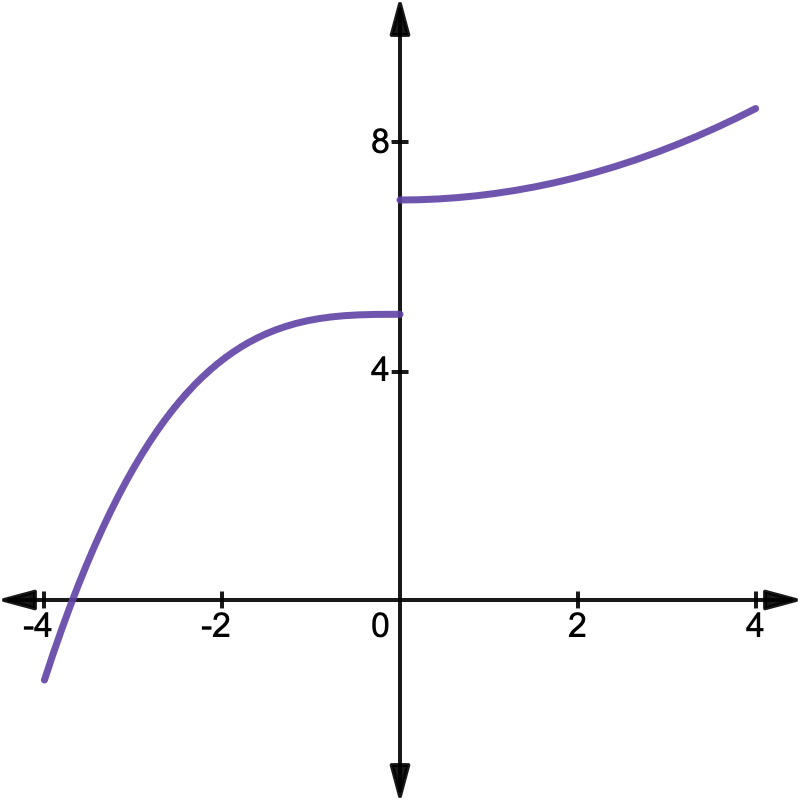
\includegraphics[scale=0.25]{input/lim1.png}	
\end{center}

\textit{Example}.  Let's calculate the limit of the following function at $x=1$.
$$f(x)\ =\ \frac{4(x-1)}{\left|x-1\right|} $$
To calculate the left-side limit plug in a value of $x$ just a tiny bit below 1, e.g. 0.99. Similarly, to calculate the right-side limit plug in a value of $x$ just a tiny bit above 1, such as 1.01. Then we can find that:
$$\lim_{x \rightarrow 1^-} f(x) = -4$$

$$\lim_{x \rightarrow 1^+} f(x) = 4$$ 
Since the left-side and right-side limit are not equal to each other, we will say that the limit of this function does not exist at 1. The graph of this function is presented below:

\begin{center}
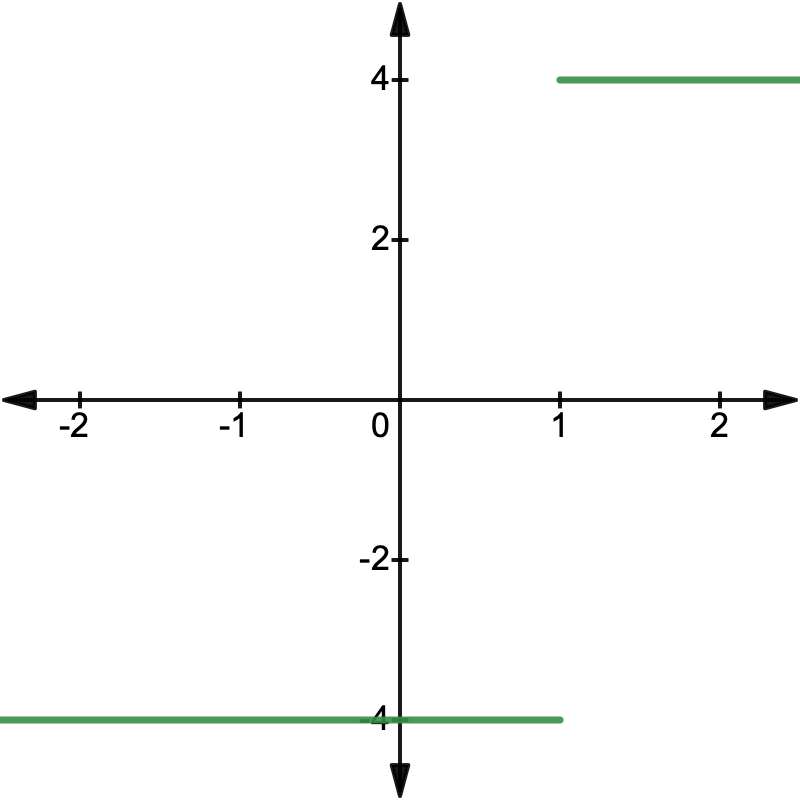
\includegraphics[scale=0.25]{input/lim2.png}	
\end{center}

%%%%%%%%%%%%%%%%%%%%%%%%%%%%%%%%%%%%%% Continuity of a Function
\section{Continuity of a Function}
A function $y=f(x)$ is said to be continuous at $a$ if the limit of $f(x)$ at $a$ exists and is equal to the value of the function at $a$ i.e.,
$$\lim _{x \rightarrow a} f(x) = f(a)$$

\textit{Example.} For the function,
$$ y = \begin{cases} 2x+1 &  \text{ if }x<1 \\
2 & \text{ if } x=1 \\
2x+1  &\text{ if }x>1 \end{cases} $$
The limit for this function exists at 1 as both the left-side limit and the right-side limit at 1 for this function is 3. But this function is not continuous because it takes value 2 when $x=1$. \\~\\

\textit{Continuity vs differentiability:} \\

$f'(x_0)$ exists if the following limit exists: 
$$  f'(x_0)= \lim_{ x \rightarrow x_0} \frac{f(x)-f(x_{0})}{x-x_0}  $$
A function $y=f(x)$ is continuous at $x_0$ if $$\lim _{x \rightarrow x_0} f(x) = f(x_0)$$
From the two definitions, we can see that continuity is a necessary condition for differentiability, but it is not a sufficient condition. In other words, if $f$ is not continuous, it implies that $f$ is not differentiable as well. But if $f$ is continuous, $f$ could either be differentiable or not. For example, the function $y = |x|$ (presented below) is continuous but not differentiable

\begin{center}
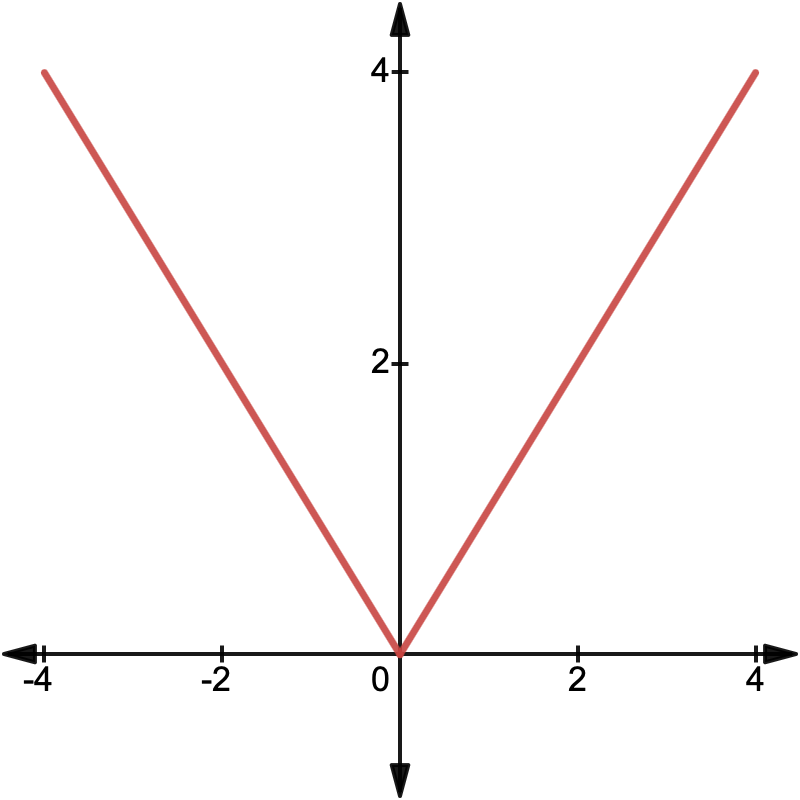
\includegraphics[scale=0.225]{input/cont_not_diff.png}
\end{center}

%%%%%%%%%%%%%%%%%%%%%%%%%%%%%%%%%%%%%% Monotonicity and inverse of a function
%\section{Monotonicity and inverse of a function}
%
%Functions that increase or decrease everywhere in their domain are called monotonic functions. Strictly increasing or decreasing functions are called strictly monotonic functions.
%\begin{itemize}
%  \item Increasing function:
%$ x_{1}>x_{2} \rightarrow f\left(x_{1}\right)\geq f\left(x_{2}\right) $ 
%\item Decreasing function:
%$ x_{1}>x_{2} \rightarrow f\left(x_{1}\right)\leq f\left(x_{2}\right) $
%\item Strictly increasing function:
%$ x_{1}>x_{2} \rightarrow f\left(x_{1}\right)>f\left(x_{2}\right) $ 
%\item Strictly decreasing function:
% $ x_{1}>x_{2} \rightarrow f\left(x_{1}\right)<f\left(x_{2}\right) $  \\
%\end{itemize}
%
%Function $y=f(x)$ has an \textit{inverse} if it is a one-to-one mapping, i.e. each value of $y$ is associated with a unique value of $x$. One-to-one mappings are unique to strictly monotonic functions. \\
%
%\textit{Definition.} For a function $y=f(x)$, the inverse function $x=f^{-1}(y)$ returns the value corresponding value of $x$ for each $y$. \\
%
%\textit{Example.} The inverse of the function $y=f(x)=2x+3$, is given by $f^{-1}(y) = (y-3)/2$ or $g(x) = (x-3)/2$. 

%%%%%%%%%%%%%%%%%%%%%%%%%%%%%%%%%%%%%% Partial Derivatives
\section{Partial Derivatives}

For a function of several variables:
$$
y=f\left(x_{1}, x_{2}, \cdots, x_{n}\right)
$$

If $x_1$ changes by $\Delta x_1$ but all other variables remain constant: 
$$
\frac{\Delta y}{\Delta x_{1}}=\frac{f\left(x_{1}+\Delta x_1, x_{2}, \cdots, x_{n}\right)-f\left(x_{1}, x_{2}, \cdots, x_{n}\right)}{\Delta x_{1}}
$$
Partial derivative of $y$ with respect to $x_i$ is defined as:
$$
\frac{\partial y}{\partial x_{i}}= f_i = \lim _{\Delta x_{i} \rightarrow 0} \frac{\Delta y}{\Delta x_{i}}
$$
Note that here, we use $\partial$ to differentiate partial derivatives from total derivatives. In particular, 
$$\left.\frac{\partial f}{\partial x_{i}} = \frac{d f}{d x_{i}} \right\vert_{\text{other variables are constant}} $$ \\

\textit{Example}. Given the production function $ Q = A K^{\alpha} L^{1-\alpha} $. \\
Marginal product of capital (MPK):
	$$\frac{\partial Q}{ \partial K} = Q_K =  \alpha A K^{\alpha-1}L^{1-\alpha}  =  \frac{\alpha Q}{K} $$

Marginal product of labor (MPL):
	$$\frac{\partial Q}{ \partial L} = Q_L = \alpha A K^{\alpha}L^{-\alpha}  =  \frac{(1-\alpha) Q}{L}$$ \\

The \textit{gradient} of a function is defined as the vector of all partial derivatives of the function:

$$ \nabla f(x_1, x_2, \cdots, x_n) = [f_1, f_2, \cdots, f_n]' $$ \\


With many functions, we can define the Jacobian matrix. Consider $n$ differentiable functions in $n$ variables that are not necessarily linear.
$$
\begin{gathered}
y_{1}=f^{1}\left(x_{1}, x_{2}, \cdots, x_{n}\right) \\
y_{2}=f^{2}\left(x_{1}, x_{2}, \cdots, x_{n}\right) \\
\cdots \\
y_{n}=f^{n}\left(x_{1}, x_{2}, \cdots, x_{n}\right)
\end{gathered}
$$ \\
The Jacobian matrix is defined
$$
J=\frac{\partial\left(y_{1}, y_{2}, \cdots, y_{n}\right)}{\partial\left(x_{1}, x_{2}, \cdots, x_{n}\right)}=\left[\begin{array}{llll}
\frac{\partial y_{1}}{\partial x_{1}} & \frac{\partial y_{1}}{\partial x_{2}} & \cdots & \frac{\partial y_{1}}{\partial x_{n}} \\
\frac{\partial y_{2}}{\partial x_{1}} & \frac{\partial y_{2}}{\partial x_{2}} & \cdots & \frac{\partial y_{2}}{\partial x_{n}} \\
\vdots & \vdots & \vdots & \vdots \\
\frac{\partial y_{n}}{\partial x_{1}} & \frac{\partial y_{n}}{\partial x_{2}} & \cdots & \frac{\partial y_{n}}{\partial x_{n}}
\end{array}\right] 
$$ \\~\\
The $n$ functions $f^{1}, f^{2}, \ldots f^{n}$ are functionally (linear or nonlinear) dependent if and only if the jacobian $|J|=0$ for all values of $x_{1}, x_{2}, \cdots, x_{n}$.

%%%%%%%%%%%%%%%%%%%%%%%%%%%%%%%%%%%%%% Differentials
\section*{Differentials}
Note that, 
$$
\Delta y \equiv\left[\frac{\Delta y}{\Delta x}\right] \Delta x
$$ 
Then for infinitesimal changes we can write,
$$
d y \equiv\left[\frac{d y}{d x}\right] d x \quad \text {or} \quad d y=f^{\prime}(x) d x
$$ 
We call $d y$ and $dx$ differentials of $y$ and $x$, respectively. We can think of $f'(x)$ as a ratio of two quantities $ dy $ and $dx$. \\

\textit{Elasticity} of function is defined as:
\[ \varepsilon = \frac{\text{Percentage change in y}}{\text{Percentage change in x}} = \frac{dy/y}{dx/x} \] 

We can calculate the elasticity by taking the derivative of $y$ with respect to $x$ as follows:
\[ \varepsilon = \frac{dy}{dx} \cdot \frac{x}{y} \]
\begin{itemize}
	\item $\varepsilon>1$, elastic
	\item $\varepsilon=1$, unit elasticity
	\item $\varepsilon<1$, inelastic \\
\end{itemize}

\textit{Example.} For the consumption function $ C = a + bY $, the elasticity is $\varepsilon = b Y/(a+bY)$. \\

For a function of $n$ variables, we can define the \textit{total differential}. For the function,  $y=f\left(x_{1}, x_{2}, \cdots, x_{n}\right)$, the total differential is given by:
\[
d f=\frac{\partial f}{\partial x_{1}} d x_{1}+\frac{\partial f}{\partial x_{2}} d x_{2}+\cdots+\frac{\partial f}{\partial x_{n}} d x_{n}=\sum_{i=1}^{n} f_{i} d x_{i}
\] \\


\textit{Example.} Consider the savings function $S=S(Y, i)$ where $S$ is savings, $Y$ is national income, and $i$ is the interest rate. Total differential is given by:
\[ 
d S=\frac{\partial S}{\partial Y} d Y+\frac{\partial S}{\partial i} d i
\] \\

The \textit{total derivative} of the $f$ with respect to $x_1$ can be obtained by dividing the total differential $df$ by $dx_1$ as follows:
\[
\frac{d f}{d x_1}=\frac{\partial f}{\partial x_{1}} +\frac{\partial f}{\partial x_{2}} \frac{d x_{2}}{d x_1}+\cdots+\frac{\partial f}{\partial x_{n}} \frac{d x_{n}}{d x_1} = f_1 +f_2\cdot \frac{d x_{2}}{d x_1}+\cdots+f_n \cdot\frac{d x_{n}}{d x_1} \]

In the case where $x_j$ does not depend on $x_1$, the term corresponding to $x_j$ will not enter the total differential as $d x_j/d x_1 = f_j= 0$. For example, if none of the other variables depend on $x_1$, the total derivative will be equal to the partial derivative. 
\[ \frac{d f}{d x_1} = \frac{\partial f}{\partial x_{1}} = f_1 \] \\

\textit{Example 1.} Suppose we have  $y = f(x_1, x_2)$ and $x_2 = g(x_1)$. In this case the total derivative of $y$ with respect to $x$ is given by:
\[ \frac{d f}{d x_1} = f_1+f_2 \cdot g'(x_1) \] \\

\textit{Example 2.} Given $y=f\left(x_{1}, x_{2}, w\right), x_{1}=g(w),$ and $x_{2}=h(w)$. The total derivative of $f$ with respect $w$ is given by:
\[ \frac{d f}{d w} = f_1 \cdot g'(w) +f_2 \cdot h'(w)  + f_3 \] \\
In this example, if instead we had $y=f(x_1, x_2)$, we could still use the definition of total derivative and just plug-in $f_3=0$ as in this case the function does not directly depend on $w$. 

%%%%%%%%%%%%%%%%%%%%%%%%%%%%%%%%%%%%%% Implicit Function Theorem
\section*{Implicit Function Theorem}

We can write an \textit{explicit} function $y=f\left(x_{1}, x_{2}, \cdots, x_{n}\right)$, as an implicit function:
\[F\left(y, x_{1}, x_{2}, \cdots, x_{n}\right)=y-f\left(x_{1}, x_{2}, \cdots, x_{n}\right)=0\] \\
\textit{Example.} For the explicit function $y = f (x_1, x_2) = x_1+3x_2-2$, we can find the implicit function $F(y, x_1, x_2) = y-x_1 -3x_2+2.$\\

However, it is not always true that for every explicit function an implicit function exists. The conditions when an implicit function exists are given by the Implicit Function Theorem stated below for the two variable case. \\

\textit{Implicit Function Theorem}

Given, $F\left(y, x \right)=0$, if the following conditions are met:
\begin{itemize}
  \item $F_y$ and $F_x$ are continuous, and
  \item at some point $x_0, y_0$ where $F(x_0,y_0) = 0$, $F_y$ is non-zero 
\end{itemize}
Then in a neighborhood around $x_0$, an implicit function exists. Moreover, this function is continuous and has continuous partial derivatives. \\

Also, when an implicit function exists, we can find its derivatives from the derivatives of the explicit function. Taking the total differential of $F\left(y, x_{1}, x_{2}, \cdots, x_{n}\right)=0$,
$$
F_{y} d y+F_{1} d x_{1}+\cdots+F_{n} d x_{n}=0 
$$

\vspace{1em}
Now suppose only $y$ and $x_{1}$ are allowed to vary, then $F_2=F_3=...=F_n=0$ and we have:
$$
F_{y} d y+F_{1} d x_{1} = 0 \quad \rightarrow \quad \frac{\partial y}{\partial x_{1}}=-\frac{F_{1}}{F_{y}} .
$$
In the simple case where the given equation is $F(y, x)=0$, the rule gives
$$
\frac{d y}{d x}=-\frac{F_{x}}{F_{y}} .
$$

\end{document}